\documentclass{ximera}
\input{../preamble.tex}
\author{}
\license{Creative Commons 4.0 By-NC-SA}
%\outcome{Compute an antiderivative using basic formulas}
\begin{document}
\begin{exercise}
Let $\mathcal{B}=\left\{\vec{v}_1, \vec{v}_2\right\}$ be a basis for the plane depicted below.  Find the coordinate vector for $\vec{x}$ with respect to $\mathcal{B}$.
\begin{center}
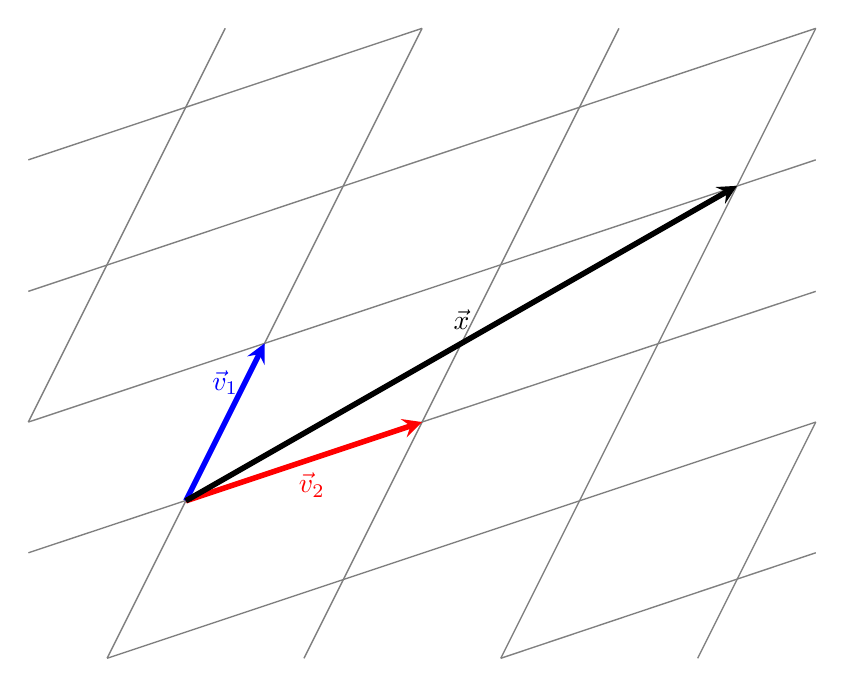
\begin{tikzpicture}[scale=1]
\draw[line width=0.5pt, gray](-2,1)--(0.5,6);  
\draw[line width=0.5pt, gray](-1,-2)--(3,6);
\draw[line width=0.5pt, gray](1.5,-2)--(5.5,6);
\draw[line width=0.5pt, gray](4,-2)--(8,6);
\draw[line width=0.5pt, gray](6.5,-2)--(8,1);
\draw[line width=0.5pt, gray](-2, 4.33)--(3,6);
\draw[line width=0.5pt, gray](-2, 2.66)--(8,6);
\draw[line width=0.5pt, gray](-2, 1)--(8,4.33);
\draw[line width=0.5pt, gray](-2, -0.66)--(8,2.66);
\draw[line width=0.5pt, gray](-1, -2)--(8,1);
\draw[line width=0.5pt, gray](4,-2)--(8,-0.66);
 \draw[line width=2pt,blue,-stealth](0,0)--(1,2);
\draw[line width=2pt,red,-stealth](0,0)--(3,1);
\draw[line width=2pt,-stealth](0,0)--(7,4);
\node[blue] at (0.5, 1.5)  (p2)    {$\vec{v}_1$};
\node[red] at (1.6, 0.2)  (p2)    {$\vec{v}_2$};
\node[] at (3.5, 2.3)  (p2)    {$\vec{x}$};
%\node[] at (-0.2, 0.2)  (p2)    {$\vec{O}$};
 \end{tikzpicture}
 \end{center}

 $$\begin{bmatrix}\answer{1}\\\answer{2}\end{bmatrix}$$

\end{exercise}
\end{document}